\documentclass{beamer}

\usepackage{fancyhdr}
\usepackage[quiet]{fontspec}
\usepackage{tikz}
\usepackage{almslides}
\usepackage{moresize}
\usepackage{hyperref}
\usepackage{svg}
\usepackage{amsmath}
\usepackage{multirow}

\usetikzlibrary{chains,decorations.pathmorphing,positioning,fit}
\usetikzlibrary{decorations.shapes,calc,backgrounds}
\usetikzlibrary{decorations.text,matrix}
\usetikzlibrary{arrows,shapes.geometric,shapes.symbols,scopes}
\usetikzlibrary{mindmap}
\usetikzlibrary{trees}

\usetheme{Hannover}

%\usecolortheme{beaver}
\setmonofont{Monaco}
\setbeamercolor{structure}{fg=cyan!90!cyan}
\setbeamerfont{block title}{size=\small}
\setbeamertemplate{frametitle}
{
	\nointerlineskip
	\begin{beamercolorbox}[sep=0.3cm,ht=1.8em,wd=\paperwidth]{frametitle}
		\vbox{}\vskip-2ex%
		\strut\insertframetitle\strut
		\vskip-0.8ex%
	\end{beamercolorbox}
}

\title{A Byte of Nginx}
\author{Sheng Yuan}

\begin{document}
    
\begin{frame}
	\centering
\includegraphics[width=0.7\textwidth]{nginx.png}
    \titlepage
\end{frame}

\begin{frame}{Contents}
    \tableofcontents
\end{frame}

\section{Introduce}
\begin{frame}
\frametitle{Introduce}
	\begin{figure}
		\centering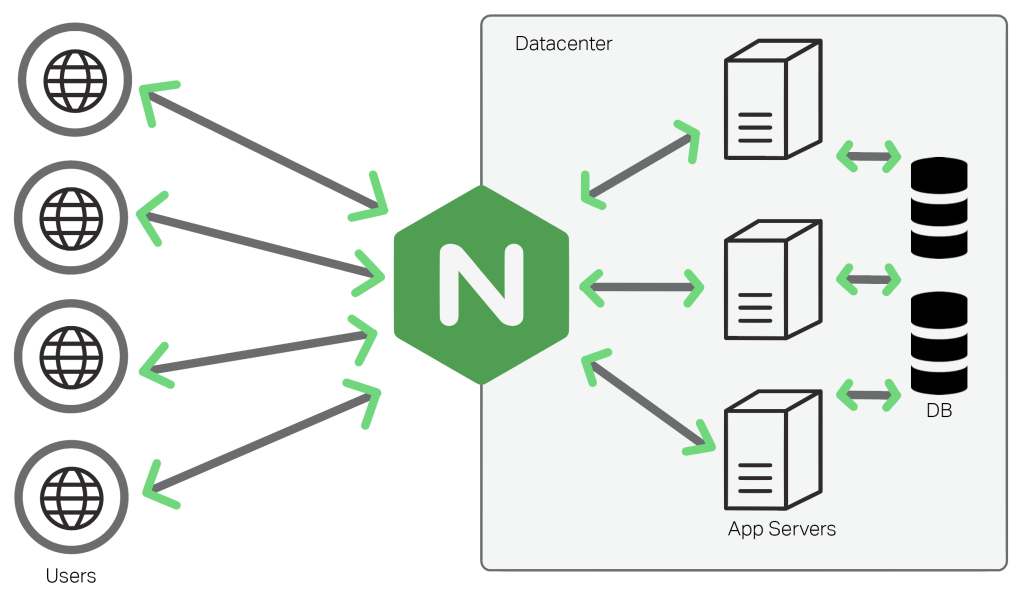
\includegraphics[width=0.7\textwidth]{nginx_architecture.png}
	\end{figure}

%	\begin{block}{Tools}
%		\begin{Alms*}
%			mongo ~~~\    mongoexport ~\ mongooplog ~\ mongos \\
%			mongod ~~\    mongofiles ~~\ mongoperf ~~\ mongostat \\
%			mongodump     mongoimport ~\ mongorestore  mongotop
%		\end{Alms*}
%	\end{block}

Nginx is a web server which can also be used as a reverse proxy, load balancer, mail proxy and HTTP cache\cite{nedelcu2015nginx}.
\end{frame}


\section{Configure and Grammar}

\begin{frame}{Basics}
\begin{minipage}[t]{0.5\textwidth}
	
	\begin{block}{Basic usage}
		\scriptsize
		\begin{Alms*}
			\$ \K{nginx} \\
			\$ \K{nginx} -s reload \\
			\$ \K{nginx}  -s stop \\
			\$ \K{nginx} -s quit \\
			\$ \K{nginx} -s reopen \\
			\$ \K{nginx} -f /conf/nginx.conf \\
			\\
			\\
			\$ service \K{nginx} start \\
			\$ service \K{nginx} stop \\
			\$ service \K{nginx} restart \\
			
			\$ kill -QUIT \$( cat /var/run/nginx.pid )
		\end{Alms*}
	\end{block}
	
\end{minipage}

\end{frame}

\begin{frame}{Config Grammar}

\begin{minipage}[t]{0.55\textwidth}
\begin{itemize}
	\item \textbf{simple directive}  the name and parameters separated by spaces and ends with a semicolon (;)
	\item \textbf{block directive}  the same structure as a simple directive, but instead of the semicolon it ends with a set of additional instructions surrounded by braces (\{ and \})
\end{itemize}
\end{minipage}
\hfil
\begin{minipage}[t]{0.4\textwidth}
		\scriptsize
		\begin{Alms*}
			\K{http} \{ \NI
			\K{server} \{ \NI	
			\K{location} \V{/} \{ \NI
			\K{root} \V{/data/www};
			\ND \} \\
			
			\K{location} \V{/images/} \{ \NI
			\K{root} \V{/data};
			\ND \}
			\ND \}
			\ND \}
		\end{Alms*}
\end{minipage}
\end{frame}

\section{Web Server}
\begin{frame}{Web Server}
\tikzstyle{every node}=[draw=black,thick,anchor=west]
\tikzstyle{selected}=[draw=red,fill=red!30]
\tikzstyle{optional}=[dashed,fill=gray!50]

\begin{minipage}[t]{0.48\textwidth}
	
\begin{block}{Simple Web Server}
	\vspace{0.01\textheight}
	\scriptsize
	\begin{Alms*}
		\K{http} \{ \NI
	\K{server} \{ \NI	
	\K{location} / \{ \NI
	\K{root} /data/www;
	\ND \} \\
	
	\K{location} /images/ \{ \NI
	\K{root} /data;
	\ND \}
	\ND \}
	\ND \}
	\\
	\end{Alms*}
\end{block}

\begin{tikzpicture}[%
grow via three points={one child at (0.5,-0.7) and
	two children at (0.5,-0.7) and (0.5,-1.4)},
edge from parent path={(\tikzparentnode.south) |- (\tikzchildnode.west)}]
\node {data}
child { node {www}}
child { node [selected] {tex}
	child { node {generic}}
%	child { node [optional] {latex}}
}
%child [missing] {}				
%child [missing] {}				
child [missing] {}				
child { node {images}};
\end{tikzpicture}

\end{minipage}
\hfil
\begin{minipage}[t]{0.48\textwidth}
	\begin{block}{Web Server with alias}
		\vspace{0.01\textheight}
		\scriptsize
		\begin{Alms*}
			\K{http} \{ \NI
			\K{server} \{ \NI
			\K{location} /static \{ \NI
			\K{alias} /opt/public;
			\ND \} \\
			\K{location} /static \{ \NI
			\K{root} /opt/public;
			\ND \}
			\ND \}
			\ND \}
			\\
		\end{Alms*}
	\end{block}

\begin{tikzpicture}[%
grow via three points={one child at (0.5,-0.7) and
	two children at (0.5,-0.7) and (0.5,-1.4)},
edge from parent path={(\tikzparentnode.south) |- (\tikzchildnode.west)}]
\node {opt}
child { node {public}
	child { node [selected] {static}
		child { node [optional] {index.html}}
		child [missing] {}
		child [missing] {}	
	}
	child [missing] {}
	child { node [optional] {index.html}}
};

\end{tikzpicture}

\end{minipage}
\end{frame}

\section{Reverse Proxy\cite{dejonghe2017nginx}}
\begin{frame}{Proxy Server}

	\begin{block}{Proxy Server}
	\vspace{0.01\textheight}
	\scriptsize
	\begin{Alms*}
		server \{ \NI
			location /debug \{ \NI
				proxy\_pass http://127.0.0.1:8000/debug;
			\ND \}
			\\
			\\
			location /static \{ \NI
				root /data/public;
			\ND \}
		\ND \}
		\\
		
	\end{Alms*}
\end{block}

\begin{block}{CORS}
	\vspace{0.01\textheight}
	\scriptsize
	\begin{Alms*}
		
		map \$request\_method \$cors\_method \{ \NI
			OPTIONS 11;
			GET 1;
			POST 1;
			default 0;
		\ND \}
		\\
		server \{ \NI
		location /api/v2 \{ \NI
		proxy\_http\_version 1.1; \\
		add\_header Access-Control-Allow-Origin *.mydomain.com; \\
		proxy\_pass http://127.0.0.1:8080/api/v2; 
		\ND \} 
		\ND \}
		\\
		
	\end{Alms*}
\end{block}

\end{frame}

\section{Load Balance}
\begin{frame}{HTTP Load Balance}
	\begin{minipage}[t]{0.8\textwidth}
		\begin{block}{Problem}
			\scriptsize
			\vspace{0.02\textheight}
			You need to distribute load between two or more HTTP servers.
		\end{block}
	
		\begin{block}{Solution}
			\vspace{0.02\textheight}
			\scriptsize
			\begin{Alms*}
				\K{upstream} backend \{ \NI
				\K{server} 10.10.12.45:80		\K{weight}=1; \\
				\K{server} app.example.com:80	\K{weight}=2; \\
				\ND \} \\
				\K{server} \{ \NI
				\K{location} / \{ \NI
				\K{proxy\_pass} http://backend;
				\ND \}
				\ND \}
			\end{Alms*}
		\end{block}
	\end{minipage}
\end{frame}


\begin{frame}{TCP Load Balance}
\begin{minipage}[t]{0.8\textwidth}
	\begin{block}{Problem}
		\vspace{0.02\textheight}
		You need to distribute load between two or more TCP servers.
	\end{block}
	
	\begin{block}{Solution}
		\vspace{0.02\textheight}
		\scriptsize
		\begin{Alms*}
			\K{stream} \{ \NI
			\K{upstream} mysql\_read \{ \NI
			\K{server} read1.example.com:3306	\K{weight}=5; \\
			\K{server} read1.example.com:3306; 	\\
			\K{server} 10.10.12.34:3306		backup;
			\ND \} \\
			\K{server} \{ \NI
			\K{listen} 3306; \\
			\K{proxy\_pass} mysql\_read;
			\ND \}
			\ND \}
		\end{Alms*}
	\end{block}
\end{minipage}
\end{frame}

\begin{frame}{Load Balancing methods}

\scriptsize
\begin{block}{Problem}
	\vspace{0.02\textheight}
	You need to choose a LB method.
\end{block}

\begin{block}{Solution}
\begin{itemize}
	\item \textcolor{cyan}{Round robin} Requests are distributed evenly across the servers, with server weights taken into consideration. This method is used by default (there is no directive for enabling it)
	\item \textcolor{cyan}{Least connections} A request is sent to the server with the least number of active connections, again with server weights taken into consideration
	\item \textcolor{cyan}{Generic hash}
	\item \textcolor{cyan}{IP hash} The server to which a request is sent is determined from the client IP address. In this case, either the first three octets of the IPv4 address or the whole IPv6 address are used to calculate the hash value. The method guarantees that requests from the same address get to the same server unless it is not available
	\item \textcolor{cyan}{Least time} Only supported in Nginx plus.
\end{itemize}
\end{block}

\end{frame}



\begin{frame}{Connection Limiting}
\scriptsize

\begin{itemize}
	\item \textcolor{cyan}{limit\_conn and limit\_conn\_zone} – Limit the number of client connections NGINX accepts, for example from a single IP address. Setting them can help prevent individual clients from opening too many connections and consuming more than their share of resources.
	\item \textcolor{cyan}{limit\_rate} – Limits the rate at which responses are transmitted to a client, per connection (so clients that open multiple connections can consume this amount of bandwidth for each connection). Setting a limit can prevent the system from being overloaded by certain clients, ensuring more even quality of service for all clients.
	\item \textcolor{cyan}{limit\_req and limit\_req\_zone} – Limit the rate of requests being processed by NGINX, which has the same benefits as setting limit\_rate. They can also improve security, especially for login pages, by limiting the request rate to a value reasonable for human users but too slow for programs trying to overwhelm your application with requests (such as bots in a DDoS attack).
	\item \textcolor{cyan}{max\_conns}  parameter to the server directive in an upstream configuration block – Sets the maximum number of simultaneous connections accepted by a server in an upstream group. Imposing a limit can help prevent the upstream servers from being overloaded. Setting the value to 0 (zero, the default) means there is no limit.
\end{itemize}
\end{frame}


\section{HTTP Caching}
\begin{frame}{Massively Scalable Content Caching}
	\begin{minipage}[t]{0.8\textwidth}
	\begin{block}{Problem}
		\vspace{0.02\textheight}
		You need to cache content and need to define where the cache is stored.
	\end{block}
	
	\begin{block}{Solution}
		\vspace{0.02\textheight}
		\scriptsize
		\begin{Alms*}
			
			\K{proxy\_cache\_path} 	/var/nginx/cache \NI
			\\
			keys\_zone=CACHE:60m
			levels=1:2 \\
			inactive=3h \\
			max\_size=20g;
			\\
			\ND \K{proxy\_cache} CACHE;
			
		\end{Alms*}
	\end{block}
\end{minipage}
\end{frame}


\section{Security and Access}
\begin{frame}{Controlling Access}
	\begin{block}{Solution}
	\vspace{0.02\textheight}
	\scriptsize
	\begin{Alms*}
		\K{location} /admin/ \{ \NI
			\K{deny} 10.0.0.1; \\
			\K{allow} 10.0.0.0/20; \\
			\K{allow} 2001:0db8::/32; \\
			\K{deny} all;
		\ND \}
	\end{Alms*}
\end{block}
\end{frame}


\begin{frame}{Force Https}
	\vspace{0.02\textheight}
	\scriptsize
	\begin{Alms*}
		\K{server}  \{ \NI
			\K{listen} \V{80}; \\
			\K{return} \V{301} https://testai.tclking.com\$request\_uri;
		\ND \}
		\\
		\\
		\K{server}  \{ \NI
		\K{listen} \V{443}; \\
		\K{ssl}          on; \\
		\K{ssl\_certificate}     /usr/share/certificates/tcl/xxx.crt; \\
		\K{ssl\_certificate\_key}  /usr/share/certificates/tcl/xxx.key; \\
		
		\K{ssl\_session\_timeout}  5m;
		\ND \}
		\\
		
		\\
		\K{add\_header} Strict-Transport-Security max-age=31536000;
	\end{Alms*}
\end{frame}



\section{Deployment and Operation}

\begin{frame}{Configuring Logs}
	\scriptsize
	\begin{Alms*}
		\K{http} \{ \NI
			\K{log\_format}  geoproxy \NI
			'[\$time\_local] \$remote\_addr ' \\
			'\$realip\_remote\_addr \$remote\_user ' \\
			'\$request\_method \$server\_protocol ' \\
			'\$scheme \$server\_name \$uri \$status ' \\
			'\$request\_time \$body\_bytes\_sent ' \\
			'\$geoip\_city\_country\_code3 \$geoip\_region ' \\
			'\$geoip\_city" \$http\_x\_forwarded\_for ' \\
			'\$upstream\_status \$upstream\_response\_time ' \\
			'"\$http\_referer" "\$http\_user\_agent"';
			\ND
			\\
		
			\K{access\_log} /var/log/nginx/access.log geoproxy buffer=32k  \\
			flush=1m; \\
			\\
			\K{error\_log} /var/log/nginx/error.log main buffer=32k \\
			flush=1m;
		\ND \}
	\end{Alms*}

	The buffer parameter of the access\_log directive denotes the size of a memory buffer that can be filled with log data before being written to disk. The flush parameter of the access\_log directive sets the longest amount of time a log can remain in a buffer before being written to disk. 
\end{frame}


\begin{frame}{Performance Tuning}
\begin{block}{Keeping Connections Open to Clients}
	\vspace{0.02\textheight}
	\scriptsize
	\begin{Alms*}
		http \{ \NI
		keepalive\_requests 320; \\
		keepalive\_timeout 300s;
		\ND \}
	\end{Alms*}
keepalive\_requests: The number of requests a client can make over a single keepalive connection. The default is 100, but a much higher value can be especially useful for testing with a load‑generation tool, which generally sends a large number of requests from a single client. \\
keepalive\_timeout: How long an idle keepalive connection remains open.
\end{block}

\begin{block}{Keeping Connections Open Upstream}
	\vspace{0.02\textheight}
	\scriptsize
	\begin{Alms*}
		proxy\_http\_version 1.1; \\
		proxy\_set\_header Connection ""; \\
		upstream backend \{ \NI
			server 10.0.0.42; \\
			server 10.0.2.56; \\
			keepalive 32;
		\ND \}
	\end{Alms*}

keepalive: The number of idle keepalive connections to an upstream server that remain open for each worker process. There is no default value.
To enable keepalive connections to upstream servers you must also include the following directives in the configuration.
\end{block}
\end{frame}


\begin{frame}{OS Tuning\cite{sharma2015nginx}}
\begin{itemize}
	\item Raising the number of open file descriptors is a more common need.
	\item Check the kernel setting for net.core.somaxconn, which is the maximum number of connections that can be queued by the kernel for NGINX to process. 
	\item Enable more ephemeral ports. 
\end{itemize}

\end{frame}

\begin{frame}{Global Parameters}

\begin{description}
	\item[worker\_processes\cite{aivaliotis2016mastering}] This is the number of worker processes
that will be started. These will handle all connections made by the clients. A good rule of thumb is to set this equal to the number of processor cores for CPU-bound loads and to multiply this number by 1.5 to 2 for I/O bound loads.
	\item[worker\_connections] This directive configures the maximum number of simultaneous connections
that a worker process may have open. This includes, but is not limited to, client connections and connections to upstream servers. This is especially important on reverse proxy servers. some additional tuning may be required at the operating system level in order to reach this number of simultaneous connections.
\end{description}

\end{frame}

%
%\begin{frame}{The Aggregation Framework}
%\begin{minipage}[t]{0.3\textwidth}
%	\begin{Alms*}
%	• \$group \\
%	• \$limit \\
%	• \$match \\
%	• \$sort \\
%	• \$unwind \\
%	• \$project \\
%	• \$lookup \\
%	\end{Alms*}
%\end{minipage}
%\hfill
%\begin{minipage}[t]{0.7\textwidth}
%	
%\end{minipage}
%\end{frame}


%\section{Python and MongoDB}
%\begin{frame}{Python and MongoDB}
%\scriptsize
%\begin{Alms*}
%	\T{int} \V{udp\_sendmsg}(\T{struct sock *}\V{sk},
%	\T{struct msghdr *}\V{msg}, \textrm{\ldots}) \\
%	\{ \NI
%	\vdots \\
%	\tikzanchor{lock 1}%
%	\only<8->{\highlight<8-9>{\V{lock\_sock}(\V{sk});} \\}%
%	\K{if} \highlight<6-8>{(\V{unlikely}(\V{sk}$→$\V{pending}))} \{ \NI
%	\highlight<5>{
%		\CCOM{Socket is already corked while preparing it} \\
%		\CCOM{\ldots\,which is an evident application bug. --ANK}
%	} \\
%	\only<9->{\highlight<9>{\V{release\_sock}(\V{sk});} \\}%
%	\V{LIMIT\_NETDEBUG}(\V{KERN\_DEBUG} \S{udp cork app bug 2}); \\
%	\highlight<6>{\K{return} -\D{EINVAL};}
%	\ND\} \\[4pt]
%	\tikzanchor{lock 2}%
%	\only<-7>{\highlight<2,7>{\V{lock\_sock}(\V{sk});} \\}%
%	\highlight<3>{%
%		\V{ret} = \V{ip\_append\_data}(\V{sk}, \V{msg}$→$\V{msg\_iov},
%		\V{ulen}, \textrm{\ldots});} \\
%	\vdots \\
%	\highlight<4>{\V{release\_sock}(\V{sk});} \\
%	\K{return} \V{ret};
%	\ND\}
%\end{Alms*}
%\end{frame}


%\begin{frame}{When to Use GridFS}
%    \begin{itemize}
%        \item When you want to keep your files and metadata automatically synced and deployed across a number of systems and facilities, you can use GridFS.
%        \item \textcolor{red}{Do not use GridFS if you need to update the content of the entire file atomically. As an alternative you can store multiple versions of each file and specify the current version of the file in the metadata. }
%    \end{itemize}
%\end{frame}


%
%\begin{frame}{Protect your Server with  Authentication}
%    MongoDB supports a role-based access control authentication model with predefined system roles and user-defined custom roles.
%    
%    \begin{minipage}[t]{0.64\textwidth}
%    	\scriptsize
%    	\begin{Alms*}
%    		> use admin \\
%    		> db.createUser(\{\NI
%    		"user":"admin", \\
%    		"pwd":"pass", \\
%    		"roles":[ \NI
%    		\{role:"readWrite", db:"admin"\}, \\
%    		\{role:"userAdminAnyDatabase", \\db:"admin"\}
%    		\ND]
%    		\ND \}) \\
%    		\$ mongod --auth \\
%    		> use admin \\
%    		> show collections \\
%    		> db.auth("admin", "pass") \\
%    		> db.getUsers() \\
%    		> use firebase
%    		
%    	\end{Alms*}
%    \end{minipage}
%	\hfill
%	\begin{minipage}[t]{0.35\textwidth}
%		\scriptsize
%		\begin{block}{User Roles}
%			\begin{itemize}
%				\item read
%				\item readWrite
%				\item userAdmin
%				\item readAnyDatabase
%				\item readWriteAnyDatabase
%				\item userAdminAnyDatabase
%				\item dbAdminAnyDatabase
%				\item clusterAdmin
%			\end{itemize}
%		\end{block}
%	\end{minipage}
%\end{frame}


\section{Conclusion}

\begin{frame}{Conclusion}
\centering
\resizebox{!}{0.8\textheight} {
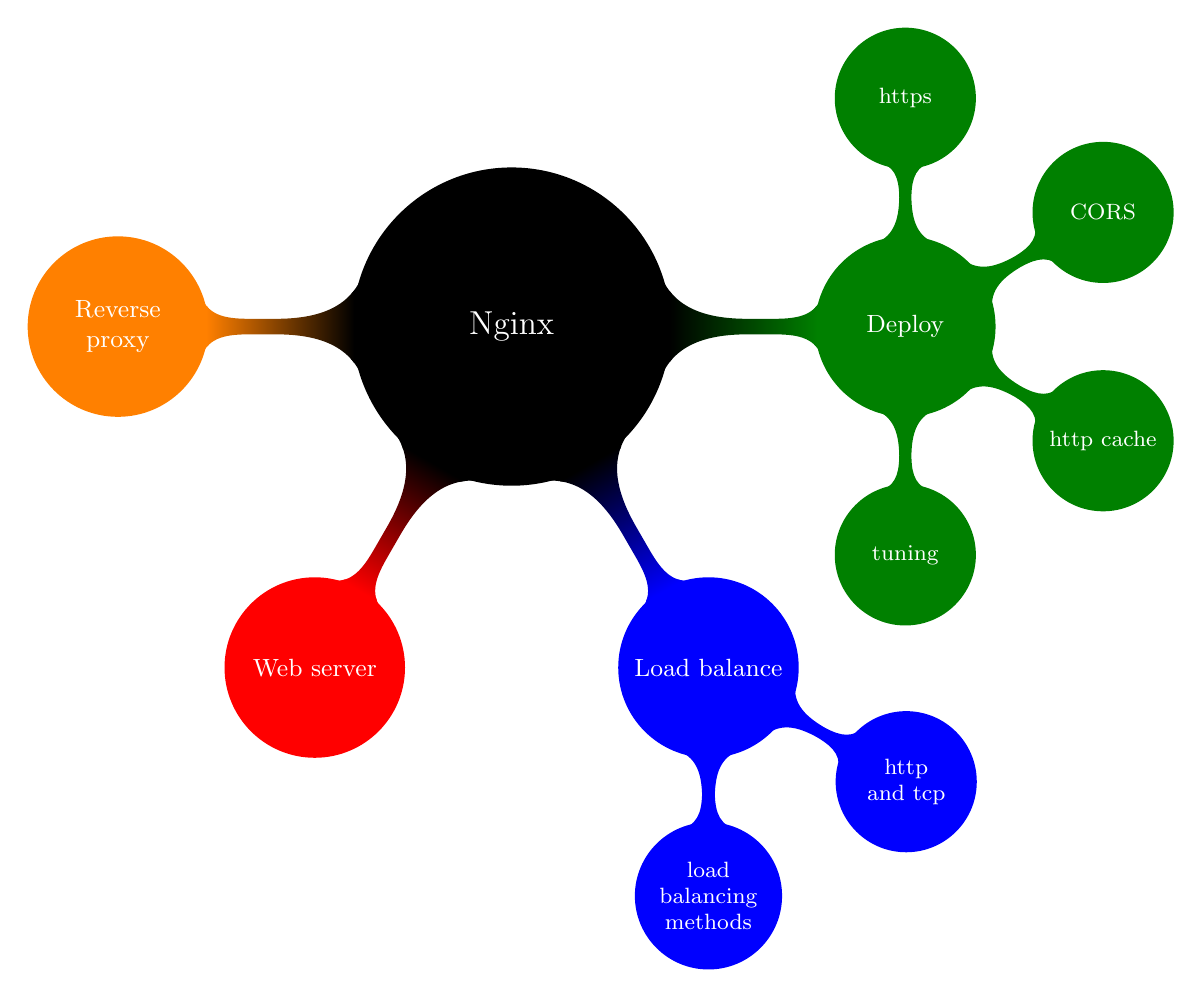
\begin{tikzpicture}
\path[mindmap,concept color=black,text=white]
node[concept] {Nginx}
[clockwise from=0]
% note that ‘sibling angle’ can only be defined in % ‘level 1 concept/.append style={}’
child[concept color=green!50!black] {
node[concept] {Deploy}
[clockwise from=90]
child { node[concept] {https} }
child { node[concept] {CORS} }
child { node[concept] {http cache} } 
child { node[concept] {tuning} }
}
child[concept color=blue] {
node[concept] {Load balance}
[clockwise from=-30]
child { node[concept] {http and tcp} } 
child { node[concept] {load balancing methods} }
}
child[concept color=red] { node[concept] {Web server} }
child[concept color=orange] { node[concept] {Reverse proxy} };
\end{tikzpicture}
}
\end{frame}

\begin{frame}{References}
\setbeamertemplate{bibliography entry title}{}
\setbeamertemplate{bibliography entry location}{}
\setbeamertemplate{bibliography entry note}{}
	\small
    \bibliography{ref}
    \bibliographystyle{plain}
\end{frame}

\end{document}
